{ \large \bfseries 2.Περιγραφή της Σχεδίασης}\\ % title 2

\begin{justify}
    Στον επεξεργαστή πολλαπλών κύκλων που πρόκειται να κατασκυεάσουμε,
    κάθε εντολή χρειάζεται διαφορετικό αριθμό κύκλων του
    ρολογίου για να ολοκληρωθεί. Για αυτό το λόγο σχεδιάστηκαν οι εξής
    καταστάσεις λειτουργίας:
\end{justify}
\begin{enumerate}
    \item {\bf\textlatin{if\_state}}:Φορτώνεται
    η εντολή από την μνήμη \textlatin{IMEM} και παιρνίεται στον καταχωρητή
    \textlatin{PC}.
    \item {\bf\textlatin{dec\_state}}:Αποκωδικοποιείται
    η εντολή που βρίσκεται στον καταχωρητή \textlatin{PC}.
    \item {\bf\textlatin{exec\_state}}:Πραγματοποείται
    ο διαχωρισμός των εντολών σε:
    \begin{enumerate}
        \item {\bf\textlatin{R-type/li/lui/addi/andi/ori}}: Υπολογισμός
        πράξης της \textlatin{ALU}.
        \item {\bf\textlatin{B/beq/bne}}: Υπολογισμός της διεύθυνσης
        της επόμενης εντολής.
        \item {\bf\textlatin{Lw/Lw/Sw}}: Υπολογισμός της διεύθυνσης
        πρόσβασης της μνήμης.
    \end{enumerate}
    \item {\bf\textlatin{mem\_state}}:Έχοντας
    την διεύθυνση πρόσβασης της μνήμης, γίνεται το \textlatin{load/store}
    αντίστοιχα.
    \item {\bf\textlatin{wb\_state}}:Αναλόγως
    την εντολή που εκτελείται γράφεται το κατάλληλο αποτέλεσμα στο αρχείο
    ακατχωρητών.
    \item {\bf\textlatin{init\_state}}: Πρακτικά κενή κατάσταση για τις εντολές
    διακλάδωσης ώστε να μην χαλάει η ροή του προγράμματος.
\end{enumerate}

\newpage

\begin{justify}
    Για να επιτευχθεί αυτός ο διαχωρισμός της εκτέλεσης
    σε διαφορετικές καταστάσεις, θα πρέπει να εισάγουμε καταχωρητές
    μευταξύ των σταδίων έτσι ώστε να αποθηκεύονται οι τιμές που
    χρειάζεται να χρησιμοποιηθούν σε κάποιο επόμενο κύκλο ρολογιού.
\end{justify}

\begin{justify}
    Προστέθηκαν οι εξής καταχωρητές:
\end{justify}

\begin{itemize}[label=\textbullet]
    \item {\bf \textlatin{Instr\_register}}: Αποθηκεύει την εντολή.
    \item {\bf \textlatin{RF\_A/RF\_B\_register}}: Αποθηκεύουν τα δεδομένα εξόδου
    του \textlatin{Register File}.
    \item {\bf \textlatin{Immed\_register}}: Αποθηκεύει την τιμή του
    \textlatin{textit{immediate}}.
    \item  {\bf \textlatin{ALU\_register}}: Αποθηκεύει το αποτέλεσμα της
    \textlatin{ALU}.
    \item  {\bf \textlatin{MEM\_register}}: Αποθηκεύει τα δεδομένα της μνήμης.
\end{itemize}


\vspace{1cm}

\begin{justify}
    Παρακάτω φαίνεται το \textlatin{DATAPATH} του επεξεργαστή 
    πολλαπλών κύκλων (με κόκκινο χρώμα οι καταχωρητές που
    προστέθηκαν): 
\end{justify}



%%PLOOOOOOOOOOOOTTTTT

\begin{figure}[h]
    \centering
    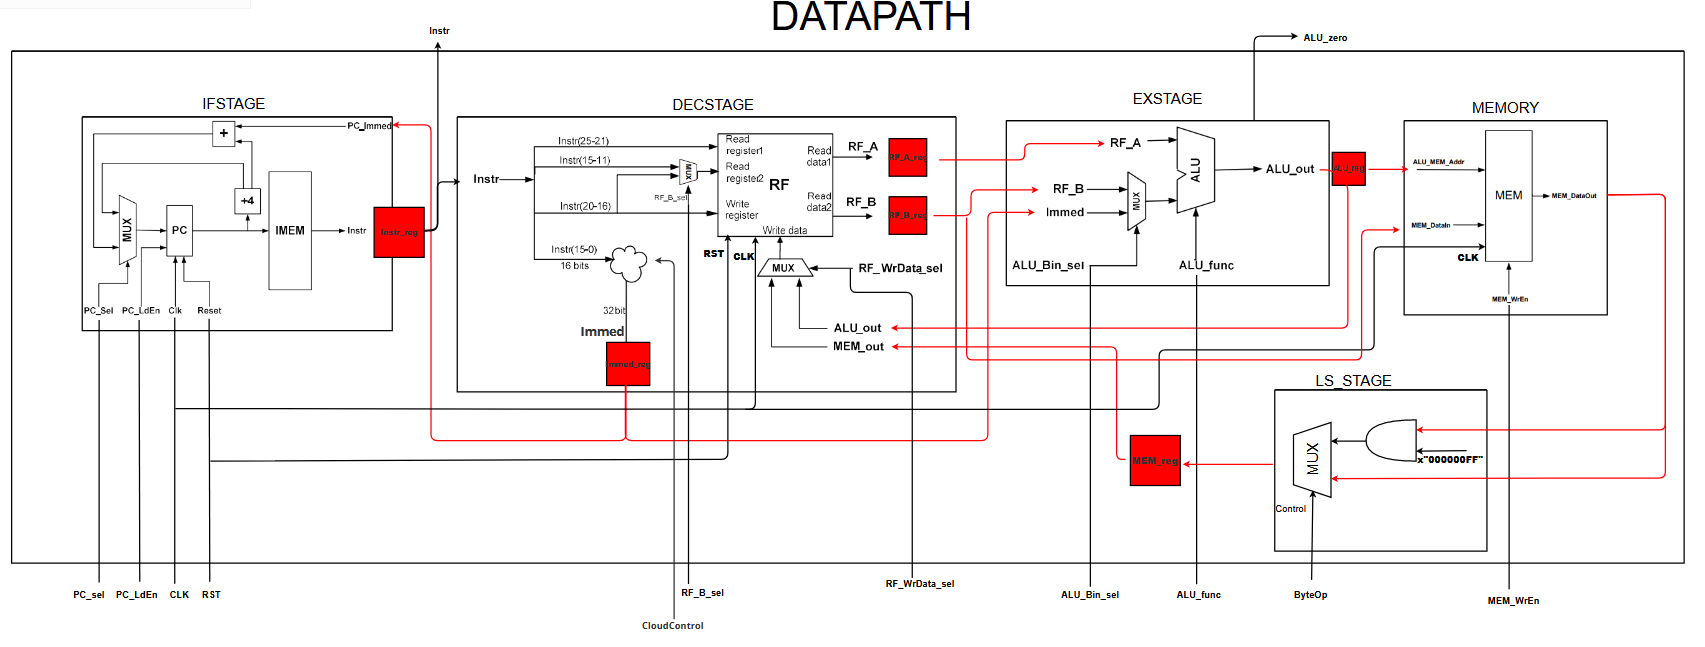
\includegraphics[width=1.1\textwidth]{IMAGES/datapath.png} % Adjust width as needed
\end{figure}

\newpage

\begin{justify}
    Τέλος, η μηχανή πεπερασμένων καταστάσεων είναι υπεύθυνη να κάνει
    τις μετβάσεις μεταξύ των σταδίων ανάλογα με την εντολή. Η μηχανή
    αλλάζει σύμφωνα με την θετική ακμή του ρολογιού και παράγει τα απαιτούμενα
    σήματα ελέγχου. Παρακάτω φαίνεται το \textlatin{State Diagram} της 
    \textlatin{FSM}:
\end{justify}


%%PLOOOOOOOOOOOOTTTTT

\begin{figure}[h]
    \centering
    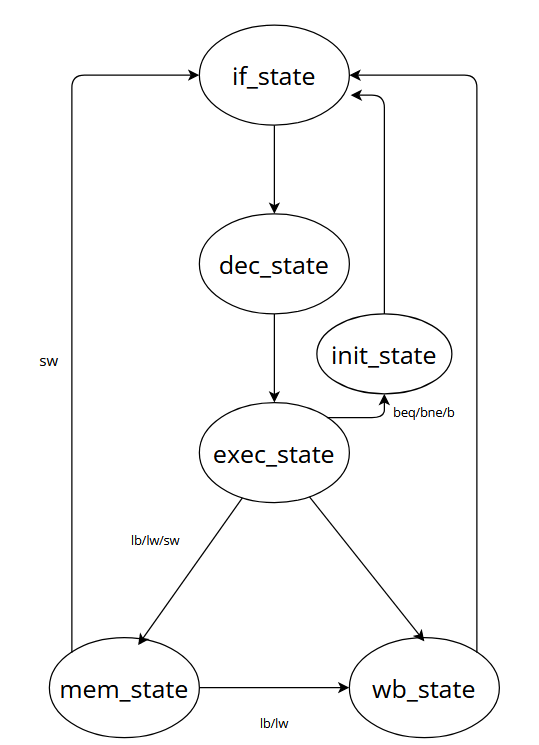
\includegraphics[width=0.6\textwidth]{IMAGES/state_di.png} % Adjust width as needed
\end{figure}
